\documentclass[utf8]{beamer} \usetheme{lfcr} % Use metropolis theme

\usepackage[brazil,english,francais]{babel}

\usepackage{natbib} \setcitestyle{round}

\usepackage{lmodern} \usepackage{datetime}

\usepackage{ulem}

\usepackage{tikz} \usetikzlibrary{shapes.geometric, arrows, shapes.misc,
  shadows.blur} \usepackage[most]{tcolorbox}

\usepackage{xcolor}

%%%% Defining colors
\definecolor{RoyalBlue}{rgb}{0.0, 0.14, 0.4} \definecolor{OliveGreen}{rgb}{0.33,
  0.42, 0.18} \definecolor{Burgundy}{rgb}{0.5, 0.0, 0.13}
\definecolor{Black}{rgb}{0.0, 0.0, 0.0} \definecolor{Blue}{rgb}{0.0, 0.53, 0.74}

\usepackage{natbib}

\usepackage{graphicx} % Allows including images
\usepackage{booktabs} % Allows the use of \toprule

\usepackage{subfig} \usepackage{stackengine}

\usepackage{float}
\usepackage{placeins} %Binds figures to its respective sections

\usepackage{cases}

\usepackage{varwidth}

\usepackage{multirow}

\usepackage{textcomp} %Text Com­n­in fonts, which pro­vie many text
% sym­ols (such as baht, bul­lt, copy­riht, mu­si­cl­icalnote,
% onequar­er, sec­ton, and yen), in the TS1 en­cocoding.

\usepackage{algpseudocode}

\usepackage{hyperref}

\usepackage{pgfgantt} % Gantt charts - for planning

\setbeamercovered{transparent} % For transparency effects with overlay commands
%
%
%
%% figure files' paths
\graphicspath{%
  {../KitPartenairesUPPA/}% logo UPPA
  {../logos/}% misc logos
  {Figures/} {Figures/VEr/} {Figures/VEz/} }

\title{Report of the ongoing experimental research on seismo-electromagnetic fields generated at saturated porous media interfaces}
\date{\today} \author{Victor MARTINS GOMES \\[3mm] Daniel BRITO (PhD supervisor)
  \\ \and H\'{e}l\`{e}ne BARUCQ (PhD co-supervisor)}
\begin{document}
\begin{frame}
  \titlepage
\end{frame}
 
%
\section{Our set-up}
\subsection{General view}
\subsection{Automation}
\begin{frame}{Automation -- general view}
  \textbf{Schema}
  \begin{center}
    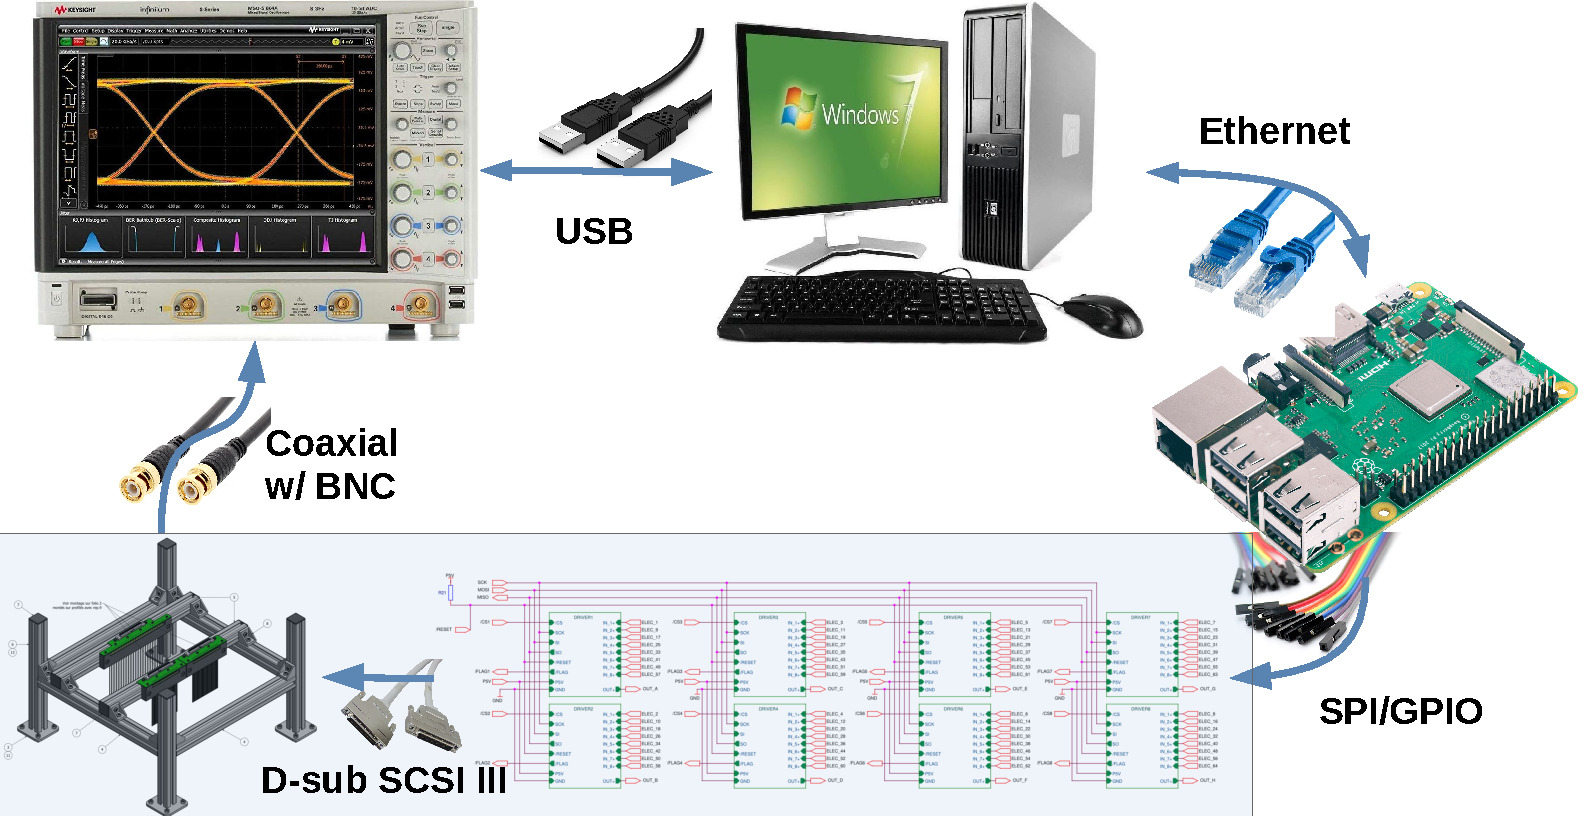
\includegraphics[width=0.85\textwidth]{schema.pdf}
  \end{center}
\end{frame}
%
\begin{frame}{Automation -- general view}
  \textbf{Main points}
  \begin{itemize}
    \item {Python-based routines and interface to control the electric acquisition}
    \item {Quicker and simpler acquisition}
    \item {Less human interaction}
    \item {Towards reproductibility}
  \end{itemize}
\end{frame}
%%%%
\begin{frame}{Automation Planning}

  \textbf{From: 2020-01-30 until 2020-03-13}

  \vspace*{0.5cm}

  \hspace*{-0.5cm} \resizebox{11.5cm}{!}{
	\begin{ganttchart}[ x unit=0.45cm, y unit title=0.7cm, y unit chart=0.9cm,
      vgrid={draw=none, dotted}, time slot format=isodate, time slot unit=day,
      calendar week text = {W\currentweek{}}, title/.append style={draw=none,
        fill=RoyalBlue!50!black}, title label font=
      \sffamily\bfseries\Large\color{white}, title label node/.append
      style={below=-1.6ex}, title left shift=.05, title right shift=-.05, title
      height=1, bar/.append style={draw=none, fill=OliveGreen!75}, bar
      height=.6, bar label font=\Large\color{black!80}, group right shift=0,
      group top shift=.6, group height=.3, group peaks height=.2, group label
      font=\sffamily\bfseries\LARGE\color{black}, bar incomplete/.append
      style={fill=Burgundy}, bar progress label font=\Large\color{Black}, group
      progress label font=\Large\color{Black}, milestone progress label
      font=\Large\color{Black}, milestone label font=\Large\color{Blue}, bar
      progress label font=\Large\color{Black}, progress=today, today=2020-02-20
      ]{2020-01-30}{2020-03-13}
      \gantttitlecalendar{year, month=name, week} \\
      \ganttbar[ bar progress label font=\Large\color{OliveGreen!75}, bar
      progress label node/.append style={right=4pt}, progress=40, bar label
      font=\LARGE\color{OliveGreen}, name=pp
      ]{Overall}{2020-01-30}{2020-03-13} \\
      \ganttset{link/.style={black, thick, -to}} \ganttbar[name=osc,
      progress=70]{Oscilloscope}{2020-01-30}{2020-03-13} \\
      \ganttbar[name=elec,
      progress=50]{Elec. card}{2020-01-30}{2020-03-13} \\
      \ganttbar[name=las,
      progress=90]{Acoustic}{2020-01-30}{2020-03-13} \\
      \ganttbar[name=tav,
      progress=30]{Tests and vali.}{2020-01-30}{2020-03-13} \\
	\end{ganttchart}
  }

  \begin{itemize}
    \item \textcolor{red}{\bf \* Proposed at 2020-02-20}
  \end{itemize}

\end{frame}
%
\begin{frame}{Automation Planning}

  \textbf{Today}

  \vspace*{0.5cm}

  \hspace*{-0.5cm} \resizebox{11.5cm}{!}{
	\begin{ganttchart}[ x unit=0.45cm, y unit title=0.7cm, y unit chart=0.9cm,
      vgrid={draw=none, dotted}, time slot format=isodate, time slot unit=day,
      calendar week text = {W\currentweek{}}, title/.append style={draw=none,
        fill=RoyalBlue!50!black}, title label font=
      \sffamily\bfseries\Large\color{white}, title label node/.append
      style={below=-1.6ex}, title left shift=.05, title right shift=-.05, title
      height=1, bar/.append style={draw=none, fill=OliveGreen!75}, bar
      height=.6, bar label font=\Large\color{black!80}, group right shift=0,
      group top shift=.6, group height=.3, group peaks height=.2, group label
      font=\sffamily\bfseries\LARGE\color{black}, bar incomplete/.append
      style={fill=Burgundy}, bar progress label font=\Large\color{Black}, group
      progress label font=\Large\color{Black}, milestone progress label
      font=\Large\color{Black}, milestone label font=\Large\color{Blue}, bar
      progress label font=\Large\color{Black}, progress=today, today=2020-04-24
      ]{2020-01-30}{2020-04-24}
      \gantttitlecalendar{year, month=name, week} \\
      \ganttbar[ bar progress label font=\Large\color{OliveGreen!75}, bar
      progress label node/.append style={right=4pt}, progress=80, bar label
      font=\LARGE\color{OliveGreen}, name=pp
      ]{Overall}{2020-01-30}{2020-04-24} \\
      \ganttset{link/.style={black, thick, -to}} \ganttbar[name=osc,
      progress=90]{Oscilloscope}{2020-01-30}{2020-03-13} \\
      \ganttbar[name=elec,
      progress=90]{Elec. card}{2020-01-30}{2020-03-13} \\
      \ganttlinkedbar[name=spi,
      progress=100]{SPI connection}{2020-02-20}{2020-02-28}\\
      \ganttlinkedbar[name=tnoise,
      progress=100]{Transformer noise}{2020-03-02}{2020-03-11}\\
      \ganttlinkedbar[name=eletr,
      progress=50]{Electrodes}{2020-03-02}{2020-03-16}\\
      \ganttbar[name=las,
      progress=100]{Acoustic}{2020-01-30}{2020-03-13} \\
      \ganttbar[name=tav,
      progress=85]{Tests and vali.}{2020-01-30}{2020-04-24} \\
	\end{ganttchart}
  }

\end{frame}
%
\begin{frame}{Automation Planning}
  \textbf{Points:}
  \begin{itemize}
    \item {Oscilloscope connection has no easy-to-use user interface.
      Possibility of bugs I have not yet seen.}
    \item {Control over GPIO pins works but SPI is not quite clear.
      \begin{itemize}
        \item {The right cable config.}
        \item {What 8-bit message do I send to change drivers/relays.}
      \end{itemize}}
    \item {Oscilloscope control could be done with LabView to make it easier.}
  \end{itemize}
\end{frame}
%
\begin{frame}{Tests to be performed}
  \begin{itemize}
    \item Check if all relays work properly - \textcolor{blue}{DONE}
    \item Test box attenuation/plastic velocity/etc \textcolor{blue}{ONGOING}
    \item Water-filled box with dipole source to check electrodes' beahviour to
      electromagnetic sources
    \item Sand-filled box
    \item Sensitivity to the Layer response
  \end{itemize}
\end{frame}
%
\begin{frame}{Perspectives to new experimentl setup}
  \textbf{General:}
  \begin{enumerate}
    \item Greater SNR;
    \item Faster acquisition
    \item Greater spatial precision of electric measurements due to more rigid
      electrodes;
    \item Ensure repeatability;
    \item More precision when studying the converted wave.
  \end{enumerate}
\end{frame}
%%%%%%%%%%%%%%%%%%%%%%%%%%%%%%%%%%%%%%%%%%%%%%%%%%%%%%%%%%%%%%%%%%%%%%%%%
  
  %%%%%%%%%%%%%%%%%%%%%%%
% DO NOT CHANGE BELOW %
  %%%%%%%%%%%%%%%%%%%%%%%
\begin{frame}{}
  \centering
  \begin{beamercolorbox}[wd=\paperwidth, ht=1.2cm]{frametitle}
    \begin{tikzpicture}
      \useasboundingbox(0,0) rectangle(\the\paperwidth,1.5); {
        \draw[preaction={fill=black,opacity=.4,transform
          canvas={xshift=0.0mm,yshift=-0.5mm}}][draw=white,fill=myblue]
        (-0.1,-1) -- (-0.1,1.5) -- (19,1.5) -- (19,-0.25); \node[anchor=base] at
        (6.12875,0) {\usebeamerfont{frametitle}\huge Thank you for your
          attention!}; }
    \end{tikzpicture}
  \end{beamercolorbox}
\end{frame}

\end{document}
